\chapter{Diagrama Base de Datos}
\label{ape:diag}

\begin{figure}[h]
\centering
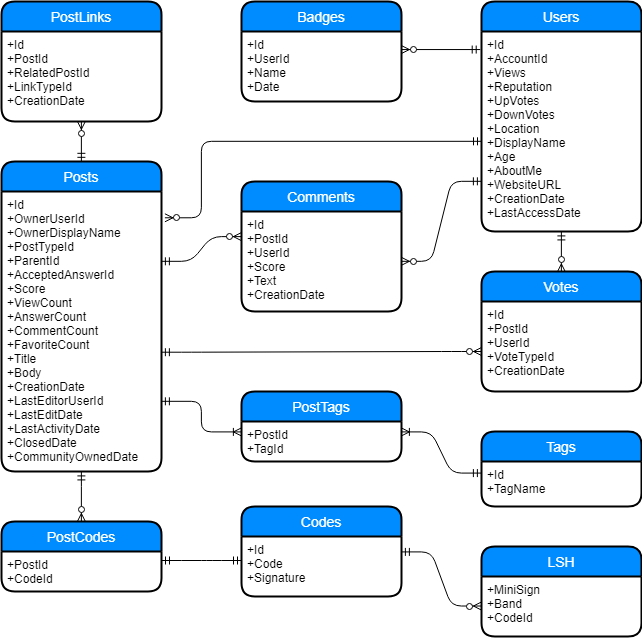
\includegraphics[width=36em]{img/er.png}
\caption{Diagrama Entidad-Relación}
\label{fig:er}
\end{figure}

%Se puede encontrar el esquema general de la base de datos en el siguiente enlace:

%\url{https://meta.stackexchange.com/questions/2677/database-schema-documentation-for-the-public-data-dump-and-sede}

\begin{table}[h]
\caption{Campos de la Tabla Badges.}
\centering
\begin{tabular}{ccc}
\hline
Nombre & Tipo & Descripción \\
\hline
Id & INTEGER & Clave primaria \\
UserId & INTEGER & Usuario asociado \\
Name & TEXT & Nombre de la medalla \\
Date & TIMESTAMP & Fecha de creación \\
\hline
\end{tabular}
\end{table}

\begin{table}[h]
\caption{Campos de la Tabla Comments.}
\centering
\begin{tabular}{ccc}
\hline
Nombre & Tipo & Descripción \\
\hline
Id & INTEGER & Clave primaria \\
PostId & INTEGER & Tópico asociado \\
UserId & INTEGER & Usuario asociado \\ 
Score & INTEGER & Puntación del comentario \\ 
Text & TEXT & Contenido del comentario \\
CreationDate & TIMESTAMP & Fecha de creación \\
\hline
\end{tabular}
\end{table}

\begin{table}[h]
\caption{Campos de la Tabla Posts.}
\centering
\begin{tabular}{ccc}
\hline
Nombre & Tipo & Descripción \\
\hline
Id & INTEGER & Clave primaria \\
OwnerUserId & INTEGER & Usuario asociado \\
OwnerDisplayName & TEXT & Nombre del usuario asociado \\
PostTypeId & INTEGER & Tipo de tópico, pregunta (1) y respuesta (2) \\ 
ParentId & INTEGER & Si es respuesta, indica pregunta asociada \\
AcceptedAnswerId & INTEGER & Si es pregunta, indica respuesta asociada \\ 
Score & INTEGER & Puntuación del tópico \\
ViewCount & INTEGER & Contador de visitas \\
AnswerCount & INTEGER & Contador de respuestas \\
CommentCount & INTEGER & Contador de comentarios \\
FavoriteCount & INTEGER & Contador de favoritos \\
Title & TEXT & Título del tópico \\
Body & TEXT & Contenido del tópico \\
CreationDate & TIMESTAMP & Fecha de creación \\
LastEditorUserId & INTEGER & Último usuario editor \\
LastEditDate & TIMESTAMP & Fecha última edición \\
LastActivityDate & TIMESTAMP & Fecha última actividad \\
ClosedDate & TIMESTAMP & Fecha al cerrar tópico \\
CommunityOwnedDate & TIMESTAMP & Fecha al asignar a la comunidad \\
\hline
\end{tabular}
\end{table}

\begin{table}[h]
\caption{Campos de la Tabla PostLinks.}
\centering
\begin{tabular}{ccc}
\hline
Nombre & Tipo & Descripción \\
\hline
Id & INTEGER & Clave primaria \\
PostId & INTEGER & Tópico asociado \\
RelatedPostId & INTEGER & Tópico relacionado asociado \\
LinkTypeId & INTEGER & Tipo de link \\
CreationDate & TIMESTAMP & Fecha de creación \\
\hline
\end{tabular}
\end{table}

\begin{table}[h]
\caption{Campos de la Tabla Tags.}
\centering
\begin{tabular}{ccc}
\hline
Nombre & Tipo & Descripción \\
\hline
Id & INTEGER & Clave primaria \\
TagName & TEXT & Nombre de la etiqueta \\
\hline
\end{tabular}
\end{table}

\begin{table}[h]
\caption{Campos de la Tabla Users.}
\centering
\begin{tabular}{ccc}
\hline
Nombre & Tipo & Descripción \\
\hline
Id & INTEGER & Clave primaria \\
AccountId & INTEGER & Identificación de la cuenta \\
Views & INTEGER & Contador de visitas \\
Reputation & INTEGER & Reputación del usuario \\
UpVotes & INTEGER & Votos positivos \\
DownVotes & INTEGER & Votos negativos \\
Location & TEXT & Localización \\
DisplayName & TEXT & Nombre del usuario \\
Age & INTEGER & Edad usuario \\
AboutMe & TEXT & Descripción personal \\
WebsiteUrl & TEXT & Página web \\
CreationDate & TIMESTAMP & Fecha de creación\\
LastAccessDate & TIMESTAMP & Fecha último acceso \\
\hline
\end{tabular}
\end{table}

\begin{table}[h]
\caption{Campos de la Tabla Votes.}
\centering
\begin{tabular}{ccc}
\hline
Nombre & Tipo & Descripción \\
\hline
Id & INTEGER & Clave primaria \\
PostId & INTEGER & Tópico asociado \\
UserId & INTEGER & Usuario asociado \\ 
VoteTypeId & INTEGER & Tipo de voto \\
CreationDate & TIMESTAMP & Fecha de creación \\
\hline
\end{tabular}
\end{table}

\newpage
\newpage
\newpage
\FloatBarrier
\begin{table}[H]
\caption{Campos de la Tabla PostTags.}
\centering
\begin{tabular}{ccc}
\hline
Nombre & Tipo & Descripción \\
\hline
PostId & INTEGER & Tópico asociado \\
TagId & INTEGER & Etiqueta asociada \\ 
\hline
\end{tabular}
\end{table}

\begin{table}[H]
\caption{Campos de la Tabla PostCodes.}
\centering
\begin{tabular}{ccc}
\hline
Nombre & Tipo & Descripción \\
\hline
PostId & INTEGER & Tópico asociado \\
CodeId & INTEGER & Código asociado \\ 
\hline
\end{tabular}
\end{table}

\begin{table}[H]
\caption{Campos de la Tabla Codes.}
\centering
\begin{tabular}{ccc}
\hline
Nombre & Tipo & Descripción \\
\hline
Id & INTEGER & Clave primaria \\
Code & TEXT & Fragmento de código \\
Signature & INT[ ] & Firma del código \\
\hline
\end{tabular}
\end{table}

\begin{table}[H]
\caption{Campos de la Tabla LSH.}
\centering
\begin{tabular}{ccc}
\hline
Nombre & Tipo & Descripción \\
\hline
MiniSign & INT[ ] & Minifirma \\
Band & INTEGER & Banda correspondiente \\
CodeId & INTEGER & Fragmento de código asociado \\
\hline
\end{tabular}
\end{table}